\chapter{Schedule}

Prima di iniziare la stesura del progetto sono stati definiti i tempi previsti
per la realizzazione delle diverse componenti e per l'integrazione complessiva.
Lo schema delle attività è stato realizzato per mezzo di un diagramma Gantt,
come illustrato nella figura \ref{gantt-diagram} e \ref{gantt-table}

\begin{figure}[htp, label={gantt-diagram}]
\begin{center}
  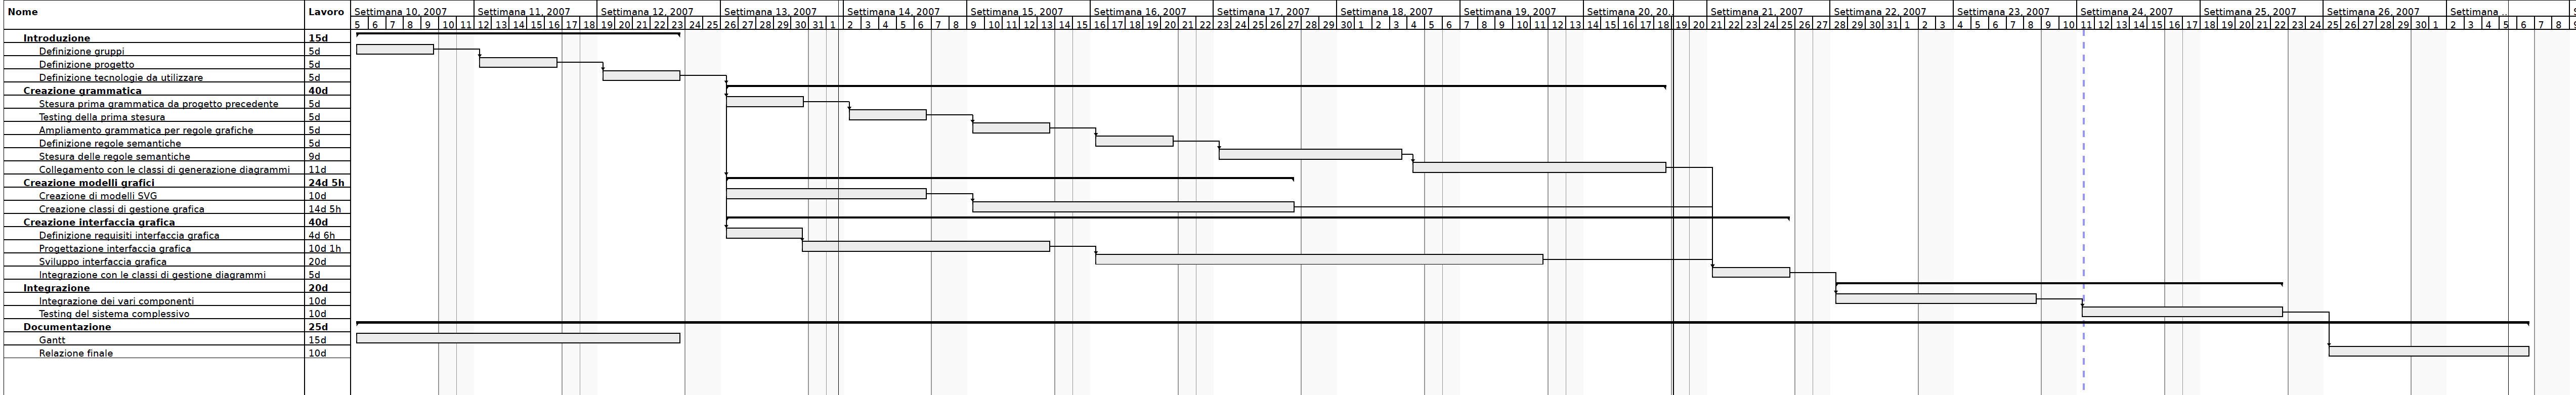
\includegraphics[width=0.9\textwidth]{img/gantt}
  \caption[labelInTOC]{Diagramma gantt}
  \label{gantt-diagram}
\end{center}
\end{figure}

\begin{figure}[htp, label={gantt-table}]
\begin{center}
  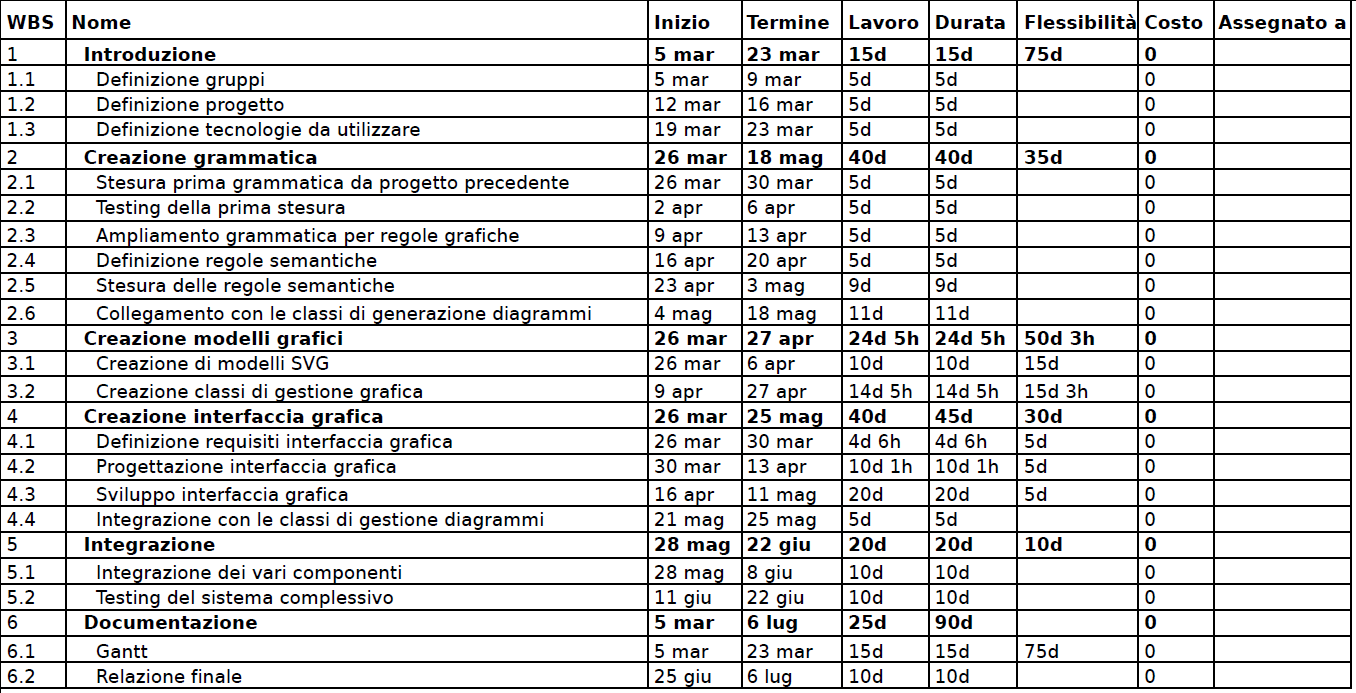
\includegraphics[width=0.9\textwidth]{img/gantt-table}
  \caption[labelInTOC]{Tabella delle attività}
  \label{gantt-table}
\end{center}
\end{figure}

La prima fase, denominata introduzione, è stata dedicata alla formazione del
gruppo di lavoro, alla stesura delle specifiche del progetto e alla scelta delle
tecnologie da utilizzare.

In seguito si è proceduto alla creazione della grammatica utilizzando la
libreria JAVACC per la creazione di compilatori in linguaggio Java. La base di
partenza è stata la grammatica realizzata per il progetto del corso di Linguaggi
e Compilatori. Successivamente alla stesura si è proceduto al testing e
all'aggiunta delle regole semantiche per il controllo della correttezza.

Parallelamente a questa fase sono stati definiti i modelli grafici da utilizzare
per l'esportazione in formato SVG e si è costruito il modello dati per
raccogliere gli oggetti contenuti nel file di modello e applicare le proprietà
provenienti dal layout per poter effettuare l'esportazione finale.

Un'altra attività svolta in contemporanea alle precedenti è stata la
realizzazione di un'interfaccia grafica che permettesse di semplificare l'uso
del compilatore da parte di un utente finale. Per questo motivo si è scelto di
realizzare un plugin per l'ambiente di sviluppo Eclipse. Tale plugin permette di
visualizzare la sintassi sia dei file di modello che di quelli di layout e si
occupa di lanciare la compilazione al momento del salvataggio.

Al termine di queste fasi si è proceduto all'integrazione dei tre componenti
ovvero compilatore, sistema di esportazione SVG e interfaccia grafica.

L'ultima attività eseguita è stata la stesura della documentazione e della
presente relazione.

Quelle di seguito sono le immagini del diagramma Gantt spezzato in quattro parti
per maggiore leggibilità.

\begin{figure}[htp, label={gantt1}]
\begin{center}
  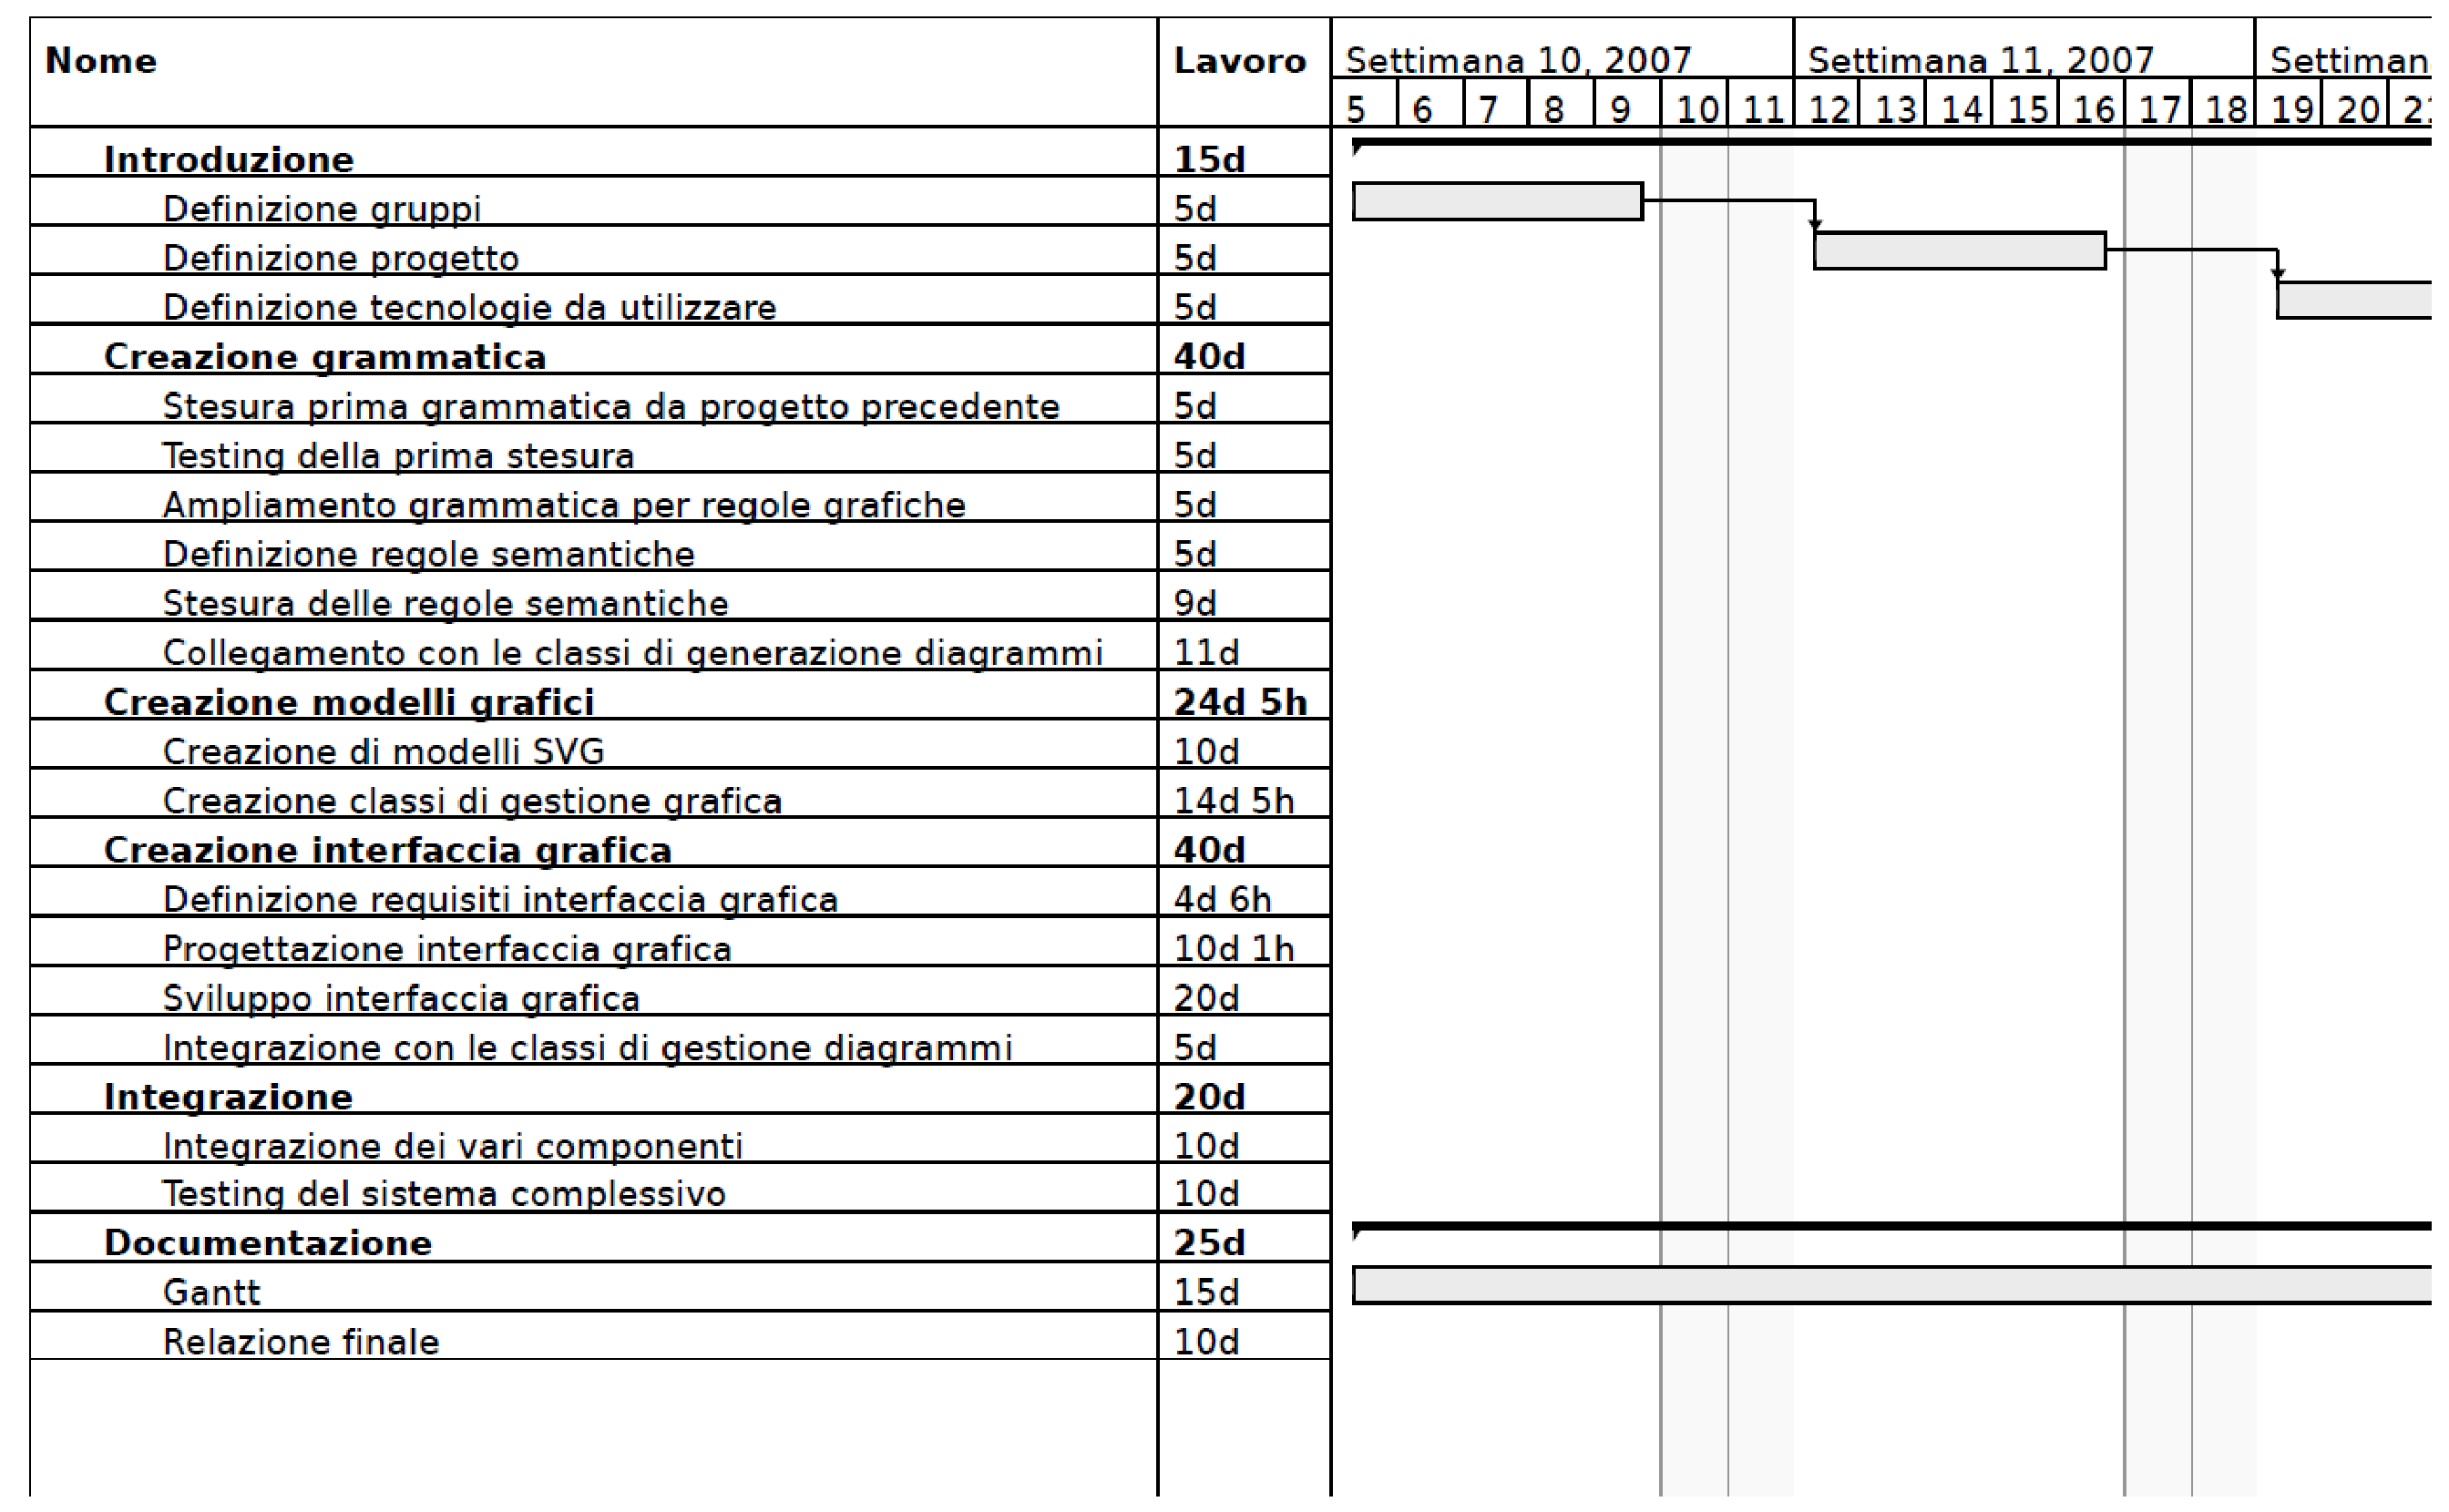
\includegraphics[width=0.9\textwidth]{img/gantt1}
  \caption[labelInTOC]{Diagramma gantt - parte 1}
  \label{gantt1}
\end{center}
\end{figure}

\begin{figure}[htp, label={gantt2}]
\begin{center}
  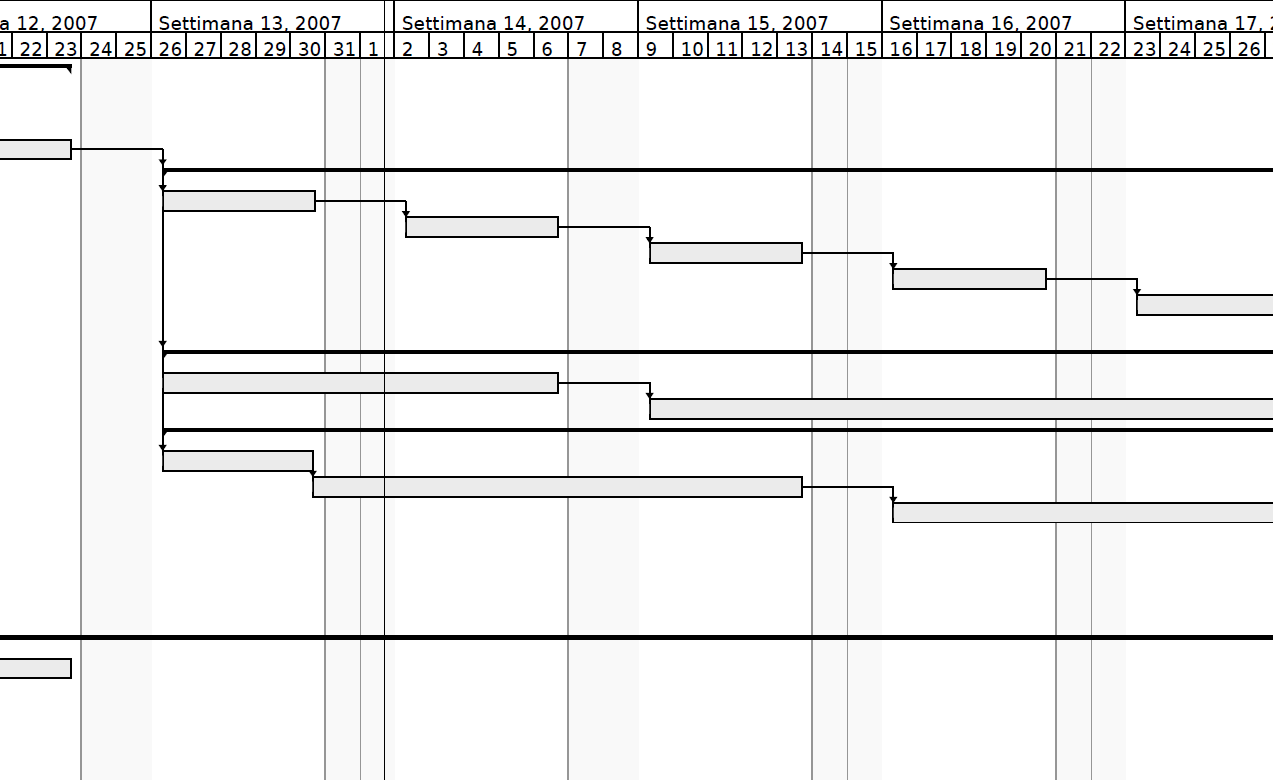
\includegraphics[width=0.9\textwidth]{img/gantt2}
  \caption[labelInTOC]{Diagramma gantt - parte 2}
  \label{gantt2}
\end{center}
\end{figure}

\begin{figure}[htp, label={gantt3}]
\begin{center}
  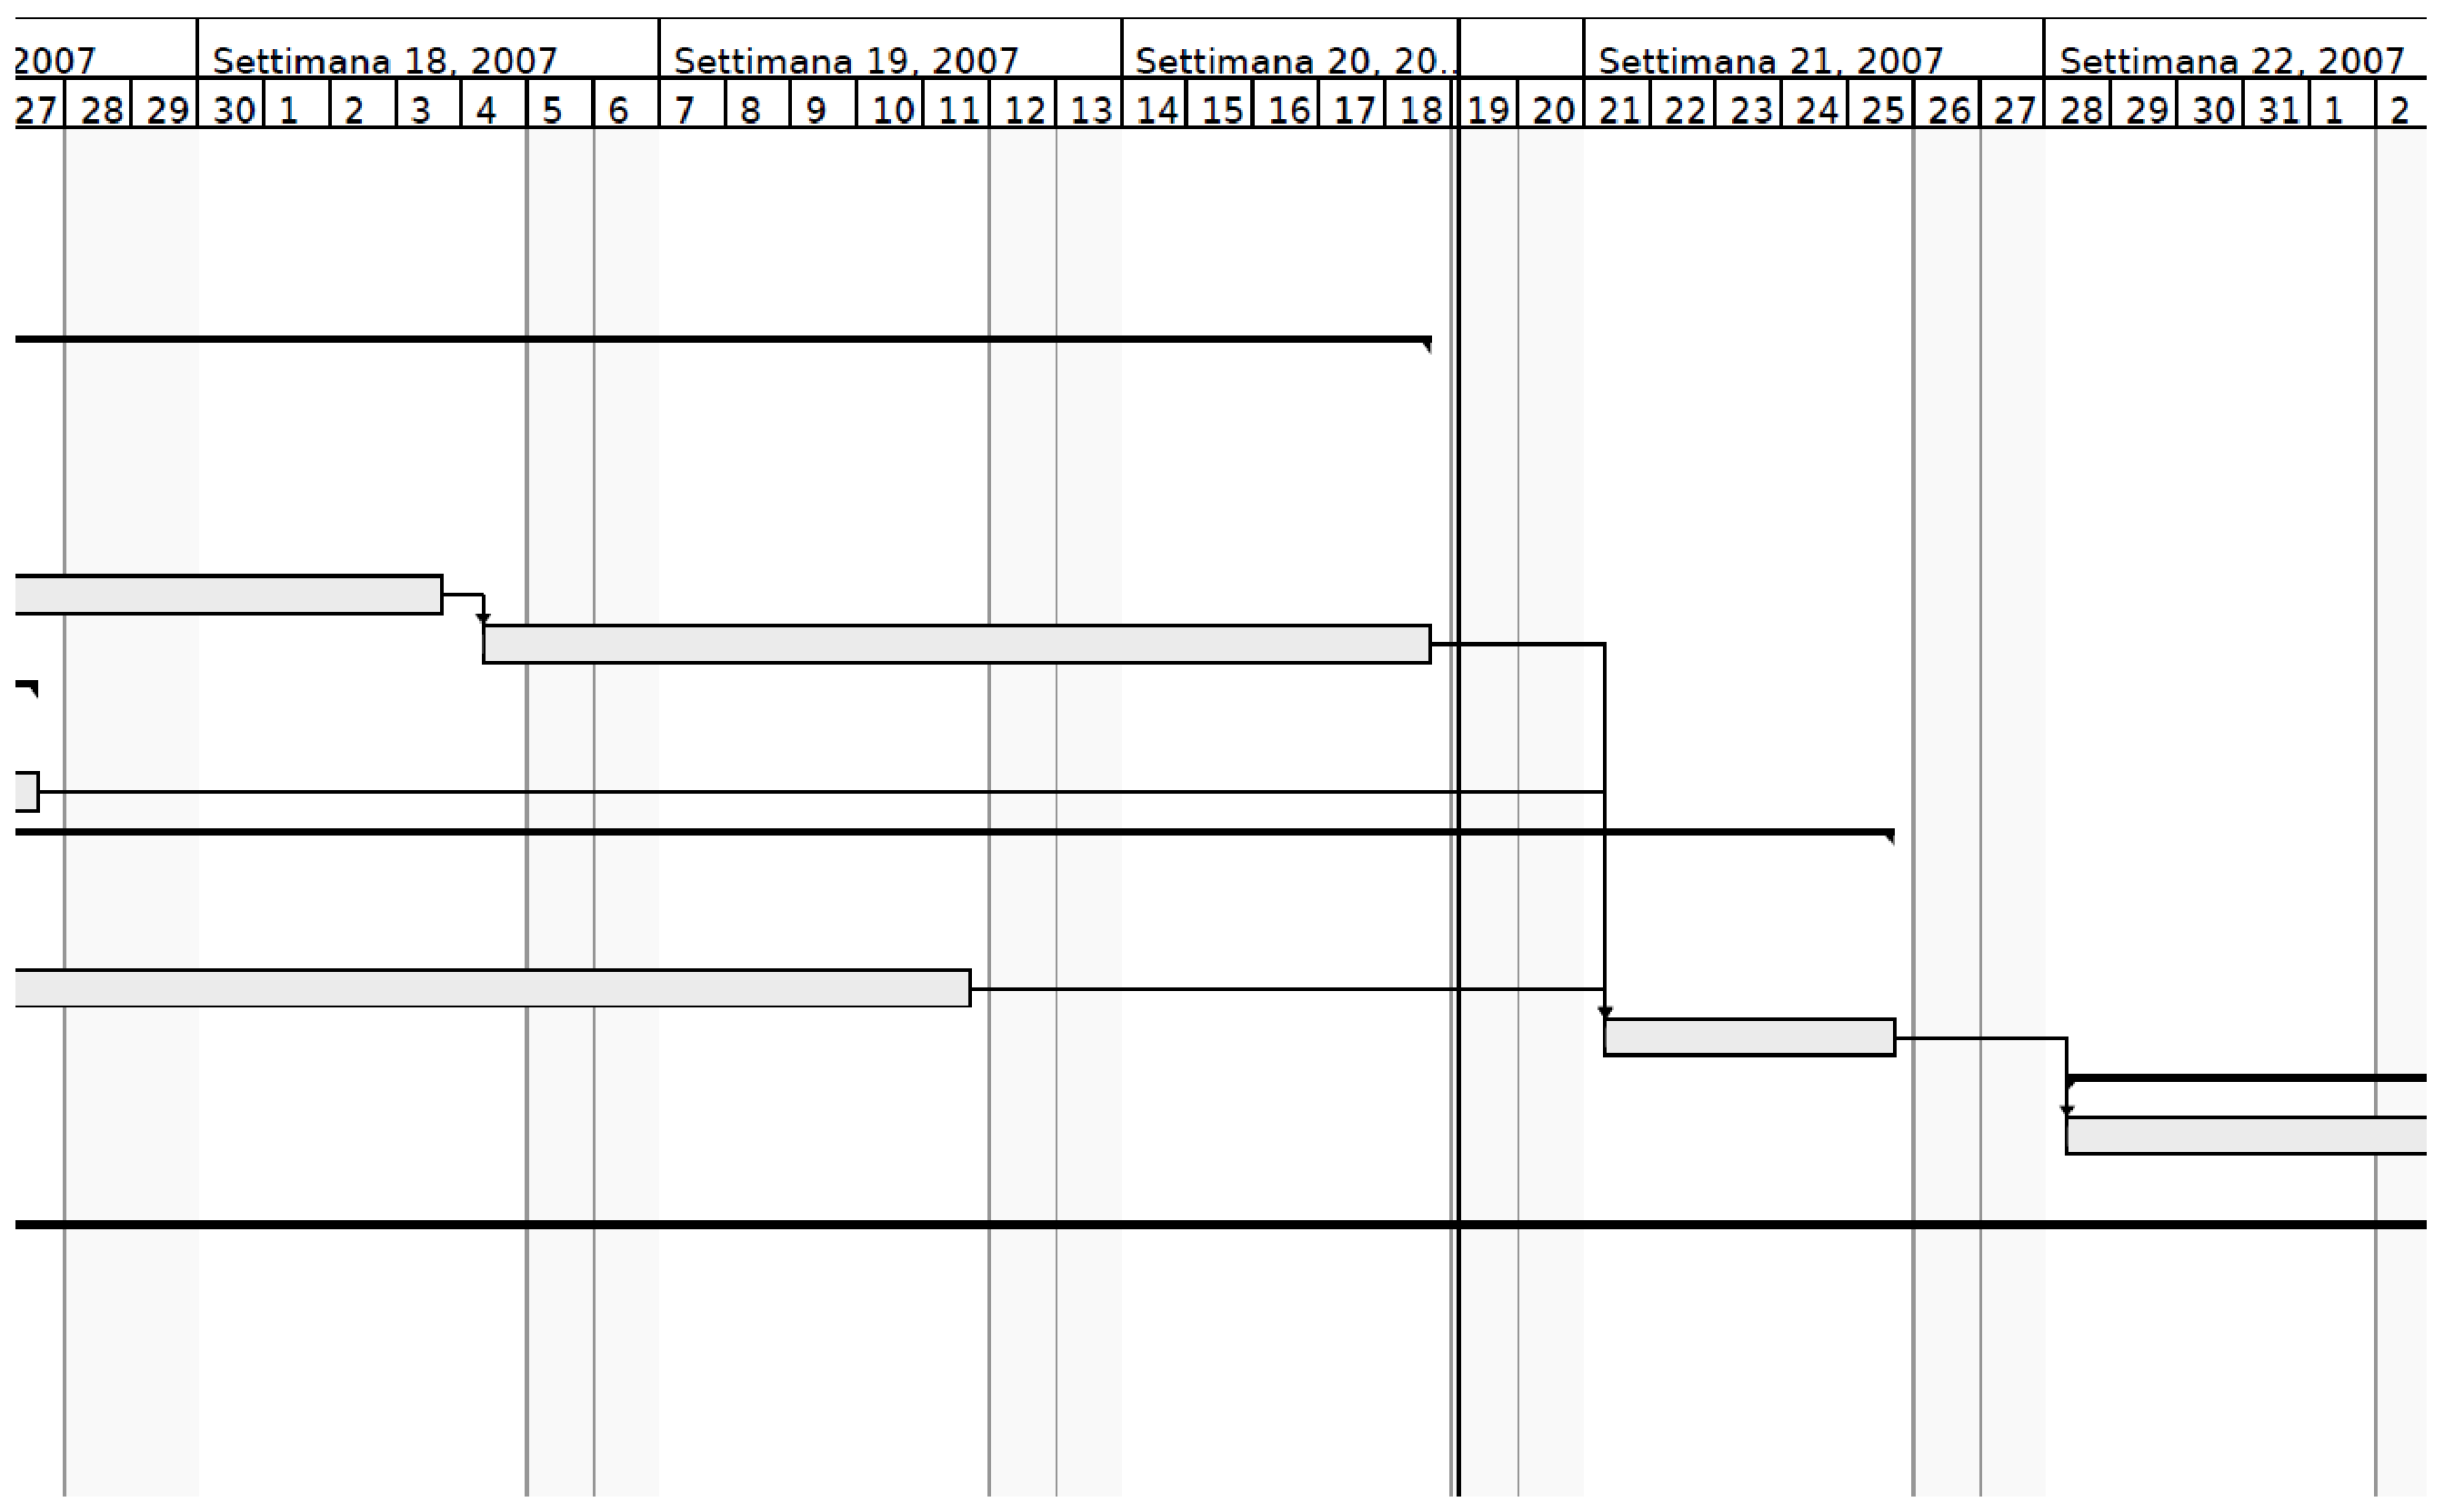
\includegraphics[width=0.9\textwidth]{img/gantt3}
  \caption[labelInTOC]{Diagramma gantt - parte 3}
  \label{gantt3}
\end{center}
\end{figure}

\begin{figure}[htp, label={gantt4}]
\begin{center}
  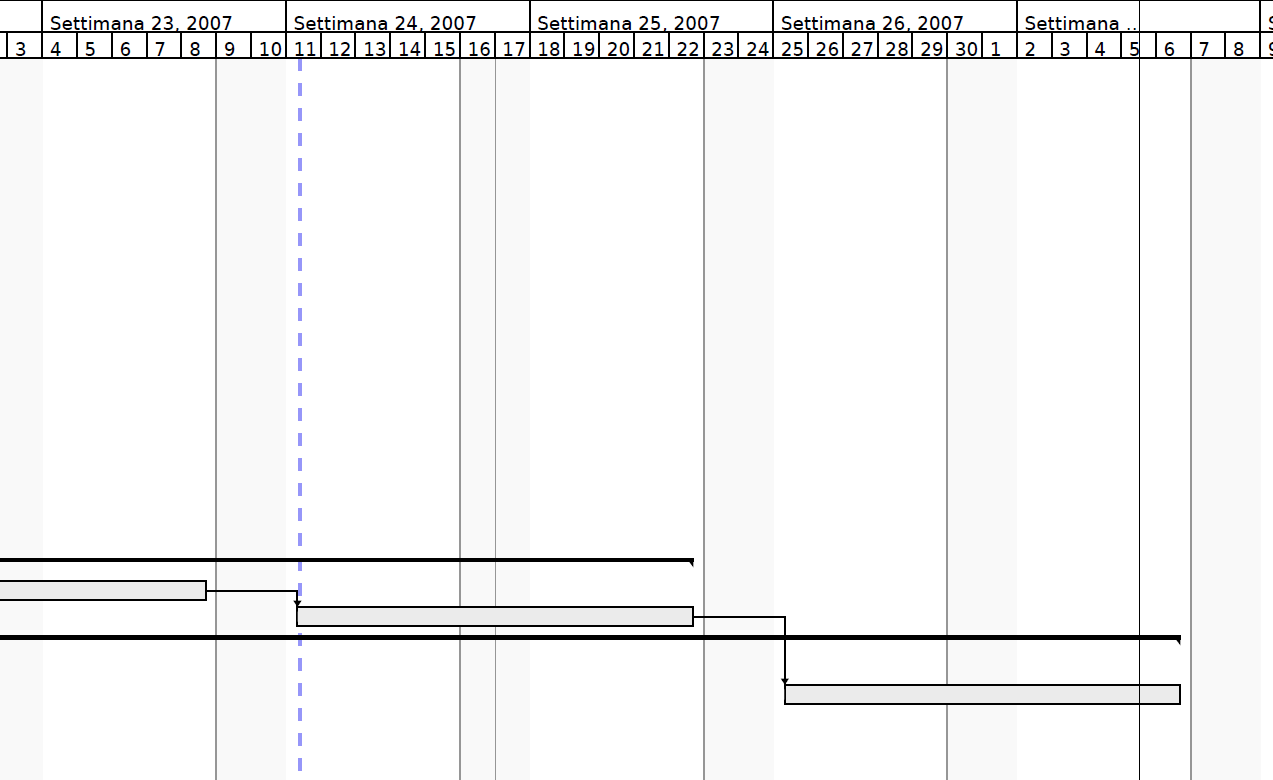
\includegraphics[width=0.9\textwidth]{img/gantt4}
  \caption[labelInTOC]{Diagramma gantt - parte 4}
  \label{gantt4}
\end{center}
\end{figure}
